\appendix
\chapter{Example Included and Excluded Trials}
\label{app}

\begin{figure}[p]
\centering
\begin{sffamily}
\large Example Included trials

\bigskip

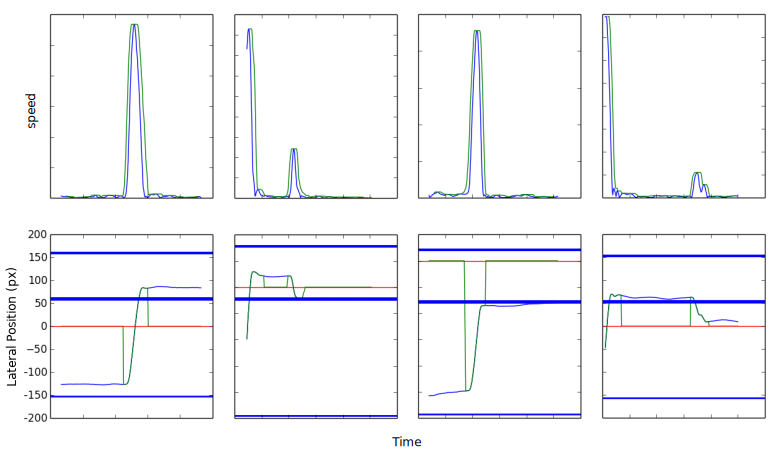
\includegraphics[width=\textwidth]{appendix/accepted}
\end{sffamily}
\caption{Figure depicts four trials selected to depict typical
examples which meet the inclusion criteria in Chapter 4. All trials
include a prominent primary saccade with clear endpoint location.}
\end{figure}

\begin{figure}[p]
\centering
\begin{sffamily}
\large Example Excluded Trials

\bigskip

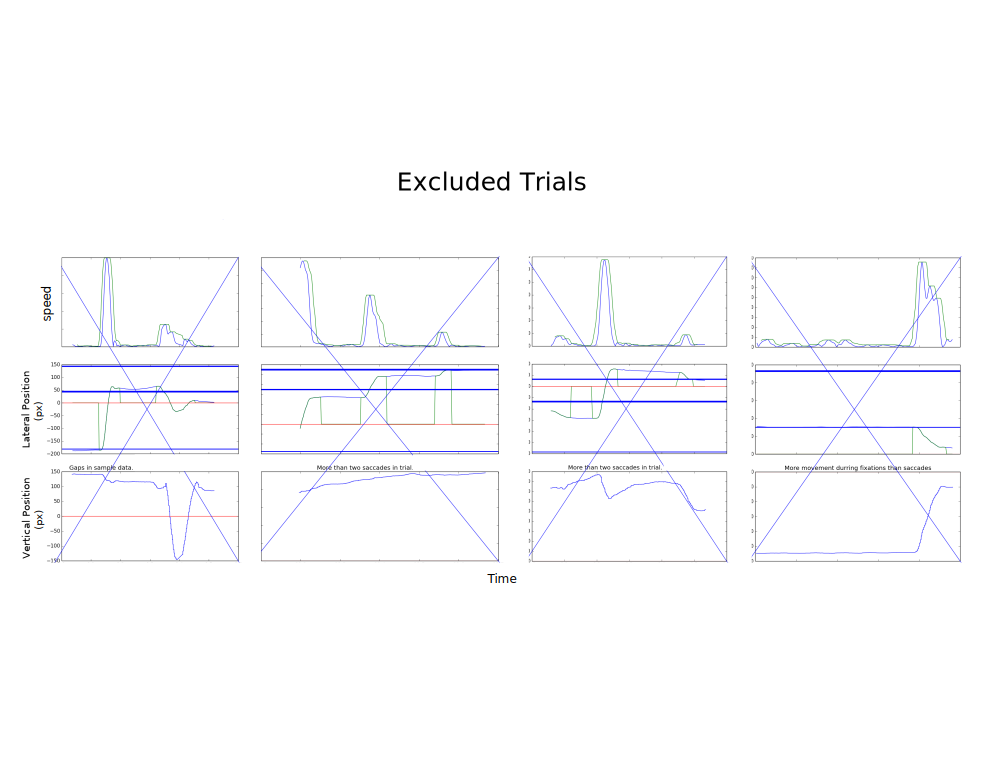
\includegraphics[width=\textwidth]{appendix/rejected}
\end{sffamily}
\caption{Figure depicts four trials selected to depict typical
examples which do not meet the inclusion criteria in Chapter 4. A) Gaps
in sample data make analysis imprecise. B and C) Trials with three or more saccades
are often unclear as to which is the primary saccade between targets or may include
distraction events or non-ballistic eye movement. 
D) large amounts of movement which does not meet saccade 
threshold often indicates drift caused by partial pupil occlusion by eyelids}
\end{figure}

\Chapter{Source Material}

Source material for this dissertation is available at <https://github.com/JasonLocklin/Dissertation>
